\documentclass[border=8pt,tikz]{standalone}
\usepackage{amsmath,amssymb}
\usepackage{tikz}
\usetikzlibrary{arrows.meta,calc,decorations.pathreplacing,patterns,shapes.geometric,positioning,shadings,plotmarks}

\begin{document}
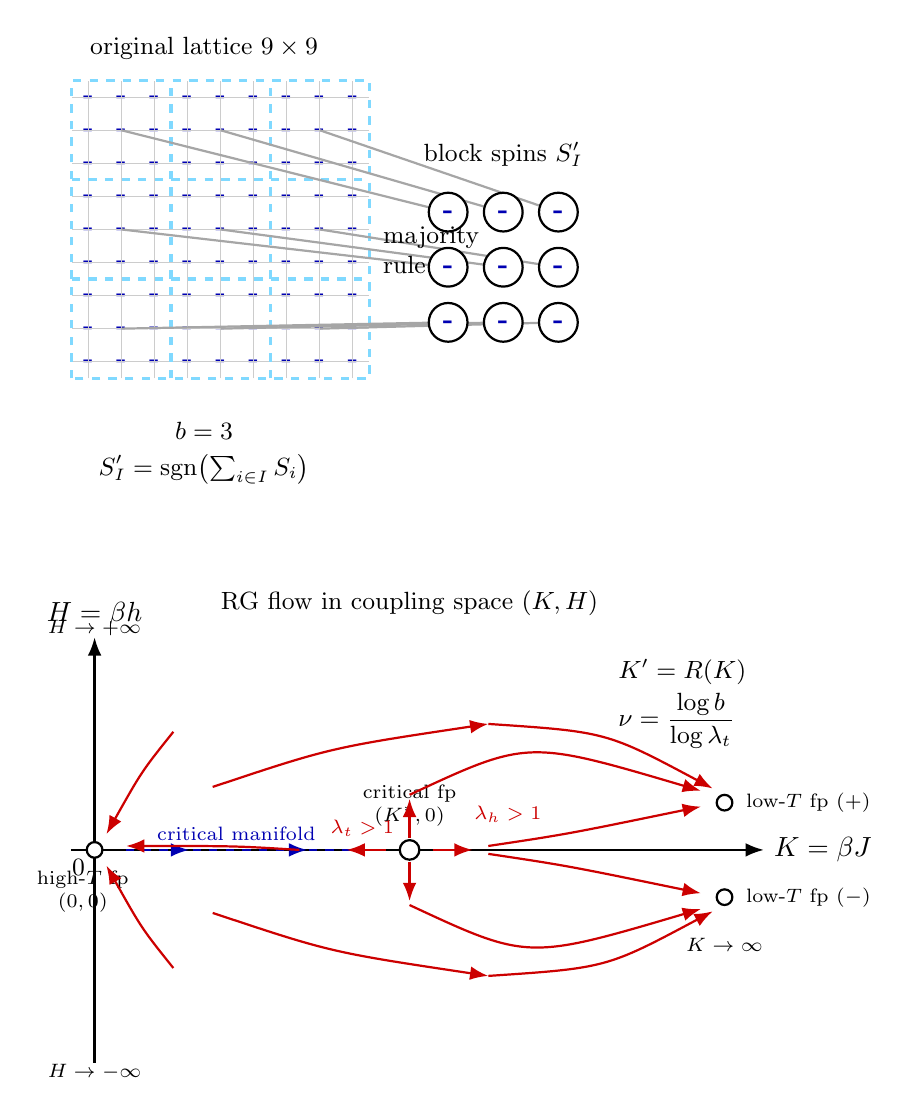
\begin{tikzpicture}[>=Latex]

% =====================================================
% TOP PANEL: 9x9 spin lattice with 3x3 block partitioning
% =====================================================

\def\cellsz{0.42}
\def\plus{\textcolor{red!70!black}{\textbf{+}}}
\def\minus{\textcolor{blue!70!black}{\textbf{-}}}

% spin pattern (9 rows, top row first, 9 spins each)
% chosen so each 3x3 block has a clear majority
% rows 1-3 form top row of blocks, rows 4-6 middle, rows 7-9 bottom
% Block (col,row): TL TM TR / ML MM MR / BL BM BR
% TL +, TM -, TR +
% ML -, MM +, MR -
% BL +, BM +, BR -

% Row 1 (top)
\def\rowA{++- --+ ++-}
\def\rowB{+-+ -+- +-+}
\def\rowC{+++ --- +-+}
% Row 2 of blocks (middle)
\def\rowD{-+- +++ ---}
\def\rowE{--- +++ -+-}
\def\rowF{-+- ++- --+}
% Row 3 of blocks (bottom)
\def\rowG{++- ++- -+-}
\def\rowH{+-+ -+- +-+}
\def\rowI{+++ -++ ---}

% draw cells with spins
% Row 1
\foreach \s/\c in {1/+,2/+,3/-,4/-,5/-,6/+,7/+,8/+,9/-} {
  \node at (\s*\cellsz, 8*\cellsz) {\ifx\c+\plus\else\minus\fi};
}
\foreach \s/\c in {1/+,2/-,3/+,4/-,5/+,6/-,7/+,8/-,9/+} {
  \node at (\s*\cellsz, 7*\cellsz) {\ifx\c+\plus\else\minus\fi};
}
\foreach \s/\c in {1/+,2/+,3/+,4/-,5/-,6/-,7/+,8/-,9/+} {
  \node at (\s*\cellsz, 6*\cellsz) {\ifx\c+\plus\else\minus\fi};
}
% Row 2
\foreach \s/\c in {1/-,2/+,3/-,4/+,5/+,6/+,7/-,8/-,9/-} {
  \node at (\s*\cellsz, 5*\cellsz) {\ifx\c+\plus\else\minus\fi};
}
\foreach \s/\c in {1/-,2/-,3/-,4/+,5/+,6/+,7/-,8/+,9/-} {
  \node at (\s*\cellsz, 4*\cellsz) {\ifx\c+\plus\else\minus\fi};
}
\foreach \s/\c in {1/-,2/+,3/-,4/+,5/+,6/-,7/-,8/-,9/+} {
  \node at (\s*\cellsz, 3*\cellsz) {\ifx\c+\plus\else\minus\fi};
}
% Row 3
\foreach \s/\c in {1/+,2/+,3/-,4/+,5/+,6/-,7/-,8/+,9/-} {
  \node at (\s*\cellsz, 2*\cellsz) {\ifx\c+\plus\else\minus\fi};
}
\foreach \s/\c in {1/+,2/-,3/+,4/-,5/+,6/-,7/+,8/-,9/+} {
  \node at (\s*\cellsz, 1*\cellsz) {\ifx\c+\plus\else\minus\fi};
}
\foreach \s/\c in {1/+,2/+,3/+,4/-,5/+,6/+,7/-,8/-,9/-} {
  \node at (\s*\cellsz, 0*\cellsz) {\ifx\c+\plus\else\minus\fi};
}

% thin grid for individual cells
\draw[gray!40,thin] (0.5*\cellsz,-0.5*\cellsz) grid[step=\cellsz] (9.5*\cellsz,8.5*\cellsz);

% thick dashed lines for 3x3 block boundaries (light blue)
\draw[blue!30!cyan!50,very thick,dashed]
  (0.5*\cellsz,-0.5*\cellsz) rectangle (9.5*\cellsz,8.5*\cellsz);
\draw[blue!30!cyan!50,very thick,dashed]
  (3.5*\cellsz,-0.5*\cellsz) -- (3.5*\cellsz,8.5*\cellsz);
\draw[blue!30!cyan!50,very thick,dashed]
  (6.5*\cellsz,-0.5*\cellsz) -- (6.5*\cellsz,8.5*\cellsz);
\draw[blue!30!cyan!50,very thick,dashed]
  (0.5*\cellsz,2.5*\cellsz) -- (9.5*\cellsz,2.5*\cellsz);
\draw[blue!30!cyan!50,very thick,dashed]
  (0.5*\cellsz,5.5*\cellsz) -- (9.5*\cellsz,5.5*\cellsz);

% block spin output (right side, 3x3 grid of block spins)
\def\blockx{6.5}
\def\blockysz{0.55}

% arrows from each block to its block spin
% block centers in lattice coords:
% block (col,row) col in {0,1,2} -> x = 2,5,8 (cell index), y = top->bot row 0,1,2 -> y = 7,4,1
% block spin grid coords (right):
% block (col,row) -> position (\blockx + col*0.85, 8*\cellsz - row*1.5*\blockysz - some)
% I'll lay out block spins in a 3x3 cluster

% block spin majorities (computed from above pattern):
% Block TL (cols 1-3, rows top): cells:
%   row1: +,+,- ; row2: +,-,+ ; row3: +,+,+ -> 7+ 2- -> +
% Block TM (cols 4-6, rows top):
%   row1: -,-,+ ; row2: -,+,- ; row3: -,-,- -> 2+ 7- -> -
% Block TR (cols 7-9, rows top):
%   row1: +,+,- ; row2: +,-,+ ; row3: +,-,+ -> 6+ 3- -> +
% Block ML (cols 1-3, rows mid):
%   row4: -,+,- ; row5: -,-,- ; row6: -,+,- -> 2+ 7- -> -
% Block MM (cols 4-6, rows mid):
%   row4: +,+,+ ; row5: +,+,+ ; row6: +,+,- -> 8+ 1- -> +
% Block MR (cols 7-9, rows mid):
%   row4: -,-,- ; row5: -,+,- ; row6: -,-,+ -> 2+ 7- -> -
% Block BL (cols 1-3, rows bot):
%   row7: +,+,- ; row8: +,-,+ ; row9: +,+,+ -> 7+ 2- -> +
% Block BM (cols 4-6, rows bot):
%   row7: +,+,- ; row8: -,+,- ; row9: -,+,+ -> 5+ 4- -> +
% Block BR (cols 7-9, rows bot):
%   row7: -,+,- ; row8: +,-,+ ; row9: -,-,- -> 3+ 6- -> -

% block centers
\coordinate (cTL) at (2*\cellsz, 7*\cellsz);
\coordinate (cTM) at (5*\cellsz, 7*\cellsz);
\coordinate (cTR) at (8*\cellsz, 7*\cellsz);
\coordinate (cML) at (2*\cellsz, 4*\cellsz);
\coordinate (cMM) at (5*\cellsz, 4*\cellsz);
\coordinate (cMR) at (8*\cellsz, 4*\cellsz);
\coordinate (cBL) at (2*\cellsz, 1*\cellsz);
\coordinate (cBM) at (5*\cellsz, 1*\cellsz);
\coordinate (cBR) at (8*\cellsz, 1*\cellsz);

% block spin destination (3x3 cluster on the right)
\def\bsx{6.0}      % offset
\def\bsy{0.0}
\def\bsspc{0.7}

\foreach \id/\dx/\dy/\sign in {
  TL/0/2/+, TM/1/2/-, TR/2/2/+,
  ML/0/1/-, MM/1/1/+, MR/2/1/-,
  BL/0/0/+, BM/1/0/+, BR/2/0/-
}{
  \coordinate (b\id) at ({9.5*\cellsz + 1.0 + \dx*\bsspc}, {\dy*\bsspc + 0.5});
}

% draw arrows from each block center to its block spin
\foreach \id in {TL,TM,TR,ML,MM,MR,BL,BM,BR} {
  \draw[->,thick,gray!70] (c\id) -- (b\id);
}

% draw block spin circles
\foreach \id/\sign in {TL/+,TM/-,TR/+,ML/-,MM/+,MR/-,BL/+,BM/+,BR/-}{
  \node[circle,draw=black,thick,fill=white,minimum size=14pt,inner sep=0pt] at (b\id) {%
    \ifx\sign+\textcolor{red!70!black}{\textbf{+}}\else\textcolor{blue!70!black}{\textbf{-}}\fi};
}

% label for block spin lattice
\node[anchor=south] at ($(bTM) + (0,0.45)$) {\small block spins $S'_I$};

% labels for 9x9 lattice
\node[anchor=south] at (4.5*\cellsz, 8.5*\cellsz + 0.15) {\small original lattice $9 \times 9$};
\node[anchor=north,font=\small] at (4.5*\cellsz, -0.65) {$b = 3$};
\node[anchor=north,font=\small] at (4.5*\cellsz, -1.05)
  {$S'_I = \mathrm{sgn}\!\left(\sum_{i\in I} S_i\right)$};

% bracket arrow between panels
\node[anchor=west,font=\small] at ({9.5*\cellsz + 0.05}, {4*\cellsz - 0.1}) {majority};
\node[anchor=west,font=\small] at ({9.5*\cellsz + 0.05}, {4*\cellsz - 0.45}) {rule};

% =====================================================
% BOTTOM PANEL: RG flow in (K,H) plane
% =====================================================

\begin{scope}[yshift=-6.2cm,xshift=0.5cm]

% axes
\draw[->,thick] (-0.3,0) -- (8.5,0) node[right] {$K = \beta J$};
\draw[->,thick] (0,-2.7) -- (0,2.7) node[above] {$H = \beta h$};

% origin label
\node[anchor=north east,font=\small] at (0,0) {$0$};

% high-T fixed point at origin
\node[circle,draw=black,thick,fill=white,inner sep=2pt] (hT) at (0.0,0.0) {};
\node[anchor=north,font=\scriptsize,align=center] at (-0.15,-0.15) {high-$T$ fp\\$(0,0)$};

% critical fixed point in middle on the K axis
\node[circle,draw=black,thick,fill=white,inner sep=2.5pt] (cFP) at (4.0,0.0) {};
\node[anchor=south,font=\scriptsize,align=center] at (4.0,0.18) {critical fp\\$(K^*,0)$};

% low-T fixed points (large K, small H)
\node[circle,draw=black,thick,fill=white,inner sep=2pt] (lTp) at (8.0,0.6) {};
\node[circle,draw=black,thick,fill=white,inner sep=2pt] (lTm) at (8.0,-0.6) {};
\node[anchor=west,font=\scriptsize] at (8.15,0.6) {low-$T$ fp $(+)$};
\node[anchor=west,font=\scriptsize] at (8.15,-0.6) {low-$T$ fp $(-)$};

% critical manifold (stable inflow line) - blue dashed - the H=0 slow direction approaching cFP
\draw[blue!70!black,dashed,thick] (0.4,0.0) -- (3.7,0.0);
\node[blue!70!black,anchor=south,font=\scriptsize] at (1.8,0.0) {critical manifold};

% inflow arrows along critical manifold (toward cFP)
\draw[->,blue!70!black,thick] (1.0,0.0) -- (1.2,0.0);
\draw[->,blue!70!black,thick] (2.5,0.0) -- (2.7,0.0);

% relevant directions: temperature (horizontal) AWAY from cFP
% to the left: from cFP toward high-T fp (decreasing K)
\draw[->,red!80!black,thick] (3.7,0.0) -- (3.2,0.0);
\draw[->,red!80!black,thick] (2.6,0.0) .. controls (1.8,0.05) .. (0.4,0.05);
% to the right: from cFP toward larger K (toward low-T)
\draw[->,red!80!black,thick] (4.3,0.0) -- (4.8,0.0);
\draw[->,red!80!black,thick] (5.0,0.05) .. controls (6.0,0.2) .. (7.7,0.55);
\draw[->,red!80!black,thick] (5.0,-0.05) .. controls (6.0,-0.2) .. (7.7,-0.55);

% relevant magnetic field direction: vertical AWAY from cFP
\draw[->,red!80!black,thick] (4.0,0.15) -- (4.0,0.65);
\draw[->,red!80!black,thick] (4.0,-0.15) -- (4.0,-0.65);
% continuing flow upward and away (curving toward low-T fp +)
\draw[->,red!80!black,thick] (4.0,0.7) .. controls (5.5,1.4) .. (7.7,0.75);
\draw[->,red!80!black,thick] (4.0,-0.7) .. controls (5.5,-1.4) .. (7.7,-0.75);

% additional flow lines off-axis showing flow toward low-T fps
\draw[->,red!80!black,thick] (1.5,0.8) .. controls (3.0,1.3) .. (5.0,1.6);
\draw[->,red!80!black,thick] (5.0,1.6) .. controls (6.5,1.5) .. (7.85,0.78);
\draw[->,red!80!black,thick] (1.5,-0.8) .. controls (3.0,-1.3) .. (5.0,-1.6);
\draw[->,red!80!black,thick] (5.0,-1.6) .. controls (6.5,-1.5) .. (7.85,-0.78);

% flow off-axis on left side: into high-T fp
\draw[->,red!80!black,thick] (1.0,1.5) .. controls (0.6,1.0) .. (0.15,0.2);
\draw[->,red!80!black,thick] (1.0,-1.5) .. controls (0.6,-1.0) .. (0.15,-0.2);

% labels for relevant eigenvalues at critical fp
\node[font=\scriptsize,red!80!black,anchor=west] at (4.7,0.45) {$\lambda_h > 1$};
\node[font=\scriptsize,red!80!black,anchor=south] at (3.4,0.05) {$\lambda_t > 1$};

% top-right boxed formulas
\node[anchor=north east,font=\small,align=left] at (8.4,2.55)
  {$K' = R(K)$\\[2pt]$\nu = \dfrac{\log b}{\log \lambda_t}$};

% asymptote labels for axes extremes
\node[anchor=north,font=\scriptsize] at (8.0,-1.0) {$K \to \infty$};
\node[anchor=south,font=\scriptsize] at (0.0,2.6) {$H \to +\infty$};
\node[anchor=north,font=\scriptsize] at (0.0,-2.6) {$H \to -\infty$};

% panel title
\node[anchor=south,font=\small] at (4.0,2.85) {RG flow in coupling space $(K,H)$};

\end{scope}

\end{tikzpicture}
\end{document}
